\begin{figure*}[t]
  \begin{center}
    \begin{tabular}{c}
      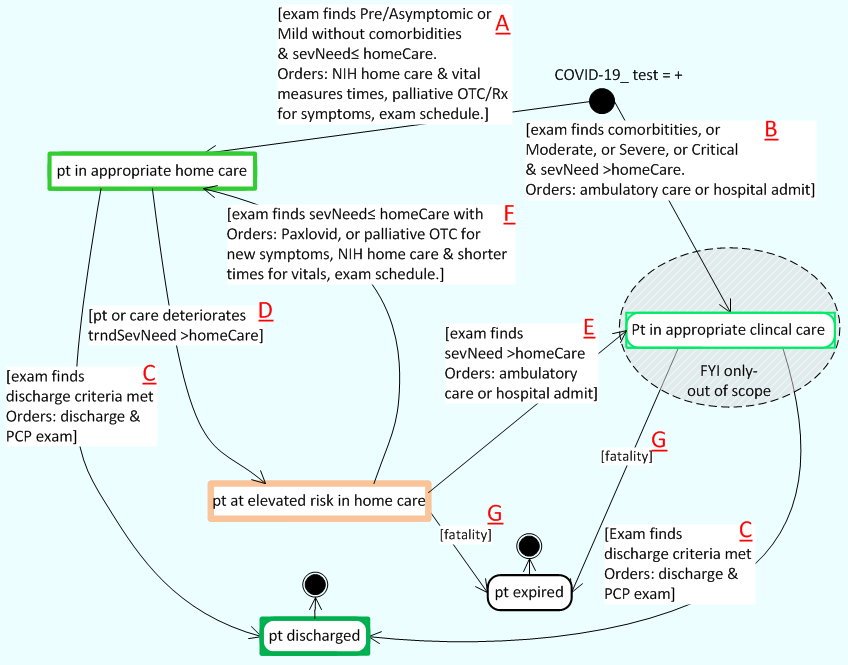
\includegraphics[scale=0.35]{cwp.png}
    \end{tabular}
  \end{center}
\caption{The CWP for remote COVID-19 patient care.}
\label{fig:cwp}
\end{figure*}

The purpose of the \phware\ is to maintain clinicians' timely awareness of patients' conditions and risk in home care to enhance patient safety with better decisions. This purpose is, however, abstract and intangible. The CWP is a declarative specification that gives precise meaning the purpose as a complex object of work shared by activities in a distributed cognitive system with allowed transformations that move the object from some initial state to a goal state.

The operational definition of actionable risk awareness for the object state in the CWP for \phware\ is the physician orders (\texttt{orders}), the actual severity of the patient an a four point scale assigned by a clinician's exam (\texttt{sevLvl}), the level of care the patient is able to maintain, either by caring for themselves or being cared for by a caregiver, while at home (\texttt{careCapLvl}), and the trending severity conjectured from the longitudinal data remotely being monitored and analyzed between exams as provided by \phware\ cloud analytics (\texttt{trndSevLvl}). 

The object state used in the CWP design as a finite state machine on actionable risk awareness for appropriate care of the patient shown in \figref{fig:cwp}.
The states are the relevant care states with the associated risks patients can occupy and the transition conditions among them. The threshold values for transitions represent an adaptation of Medicare’s four point severity-of-illness rating system to CDC’s Interim Guidance for COVID-19 home care \cite{severity,Hornbrook2005OverviewOD,cdc} where a severity level less than two is mild and a home care capability level equal to two is typical.

In the initial state (top) the patient has tested positive. The arc labeled \textbf{A} occurs when an exam shows symptoms of low severity and a provider orders home care with \phware. Outpatients remain in appropriate home care until either an exam finds discharge criteria met and ordered (\textbf{C}), or the trending severity level is greater than their care capability level (\textbf{D}). In such cases, patients are at an \emph{elevated risk} in home care. They must not remain at an elevated risk in home care because there is a possible direct path to fatality (\textbf{G}). So a near future exam must either order admission (\textbf{E}), find their risk lower than what the analytics claimed, or make their risk lower with additional prescribed interventions (\textbf{F}). Patients who are admitted to hospital may eventually be discharged back to home care (\textbf{H}) or discharged directly (\textbf{C}). 

The declarative knowledge of the CWP specifies \emph{what} workflows solving the CWP must accomplish without depending on \emph{how} they do it. In this application, the CWP motivates the design, and then when the design is ready, the CWP is the property for formal verification that must be satisfied. Conversely, it is possible to extract a CWP from workflow models in which case the intent is to discover what the system will accomplish. The genesis of the CWP for \phware\ and its validation, though an interesting problem in its own right, is outside the scope of this paper.